% !TeX root = Tesis.tex
\documentclass[12pt,fleqn,letterpaper]{scrbook}

\newcommand{\thesistitle}{Medical image segmentation in a multiple labelers
context: Application to the study of histopathology.}
\newcommand{\thesistitlees}{Segmentación de imágenes médicas en un
contexto de múltiples anotadores: Aplicación al estudio de histopatologías}

% Packages
\usepackage[pagebackref=true]{hyperref}
%\usepackage{hyperref}
\usepackage[subfigure]{tocloft}
%\usepackage[subfig]{tocloft}
%\usepackage{tocloft}
%\usepackage{tocloft}
\usepackage[utf8]{inputenc}
\usepackage[english]{babel}
\usepackage{fancyhdr}
\usepackage{epsfig}
\usepackage{epic}
\usepackage{eepic}
\usepackage{threeparttable}
\usepackage{amscd}
\usepackage{here}
\usepackage{graphicx}
\usepackage{lscape}
%\usepackage{subfigure}
\usepackage{longtable}
\usepackage{setspace}
\usepackage{array}
\usepackage{float}
\usepackage{booktabs}
\usepackage{svg}
\usepackage{minted}
\usepackage{listings}
\usepackage{xparse}
\usepackage{xstring}
\usepackage[titletoc]{appendix}
%\usepackage{subfig}
\usepackage{enumitem}
\usepackage{cancel}
\usepackage{multirow}
\usepackage{longtable}
%\usepackage{hyperref}
\usepackage{tcolorbox}
\usepackage{subfig}
\usepackage{breakcites}

\raggedbottom

% Show margins
% \usepackage{showframe}
% \renewcommand*\ShowFrameLinethickness{0.1pt}
% \renewcommand*\ShowFrameColor{\color{black!10!white}}

\usepackage{caption}
%\usepackage{subcaption}

% Math
\usepackage{amstext,amsbsy,amsopn,amsmath,eucal,amsfonts,amssymb,amsthm}

% Fonts
\usepackage{fontspec}
\setmainfont[
  Path=Fonts/Ancizar/,
  BoldFont={Ancizar-Serif-Bold.otf},
  ItalicFont={Ancizar-Serif-Regular-Italic.otf},
  BoldItalicFont={Ancizar-Serif-Bold-Italic.otf},
  %  SmallCapsFont={Ancizar-Serif-Light.otf},
  %  SlantedFont={Ancizar-Serif-Light.otf},
  %  UprightFont={Ancizar-Serif-Light.otf}
]{Ancizar-Serif-Regular.otf}
\setmonofont[
  Path=Fonts/Noto Sans Mono/,
  %  Scale=0.5
]{NotoSansMono-Regular.ttf}

\DeclareOldFontCommand{\rm}{\normalfont\rmfamily}{\mathrm}
\DeclareOldFontCommand{\sf}{\normalfont\sffamily}{\mathsf}
\DeclareOldFontCommand{\tt}{\normalfont\ttfamily}{\mathtt}
\DeclareOldFontCommand{\bf}{\normalfont\bfseries}{\mathbf}
\DeclareOldFontCommand{\it}{\normalfont\itshape}{\mathit}
\DeclareOldFontCommand{\sl}{\normalfont\slshape}{\@nomath\sl}
\DeclareOldFontCommand{\sc}{\normalfont\scshape}{\@nomath\sc}

% Titles
% \fontsize{<size>}{<bskip>}
% \titleformat{command}[shape]{format}{label}{sep}{before}[after]
\usepackage{titlesec}
% \titleformat{\chapter}{\normalfont\fontsize{200}{30}\bfseries}{\thechapter}{1em}{}
\titleformat{\section}{\normalfont\fontsize{20}{20}\bfseries}{\thesection}{1em}{}
\titleformat{\subsection}{\normalfont\fontsize{17}{17}\bfseries}{\thesubsection}{1em}{}
\titleformat{\subsubsection}{\normalfont\fontsize{14}{14}\bfseries}{\thesubsubsection}{1em}{}

% \titlespacing{command}{left spacing}{before spacing}{after spacing}[right]
\titlespacing{\section}{0pt}{2em}{1em}
\titlespacing{\subsection}{0pt}{2em}{1em}
\titlespacing{\subsubsection}{0pt}{1em}{0.5em}

% UN colors
% http://identidad.unal.edu.co/identidad-visual/b-directrices-y-especificaciones/b1-elementos-de-identidad-visual/#c1998
\usepackage{xcolor}
\definecolor{UN_primary}{RGB}{148,180,59}
\definecolor{UN_secondary}{RGB}{166,28,49}
\definecolor{UN_comp1}{RGB}{70,107,63}
\definecolor{UN_comp2}{RGB}{118,35,47}
\definecolor{UN_comp3}{RGB}{86,90,92}
\definecolor{UN_comp4}{RGB}{177,178,176}
% \definecolor{Nessa}{RGB}{1,87,155}

% Inline source code
\NewDocumentCommand{\quottable}{m}{\texttt{\bfseries\textcolor{UN_secondary}{#1}}}
\NewDocumentCommand{\quot}{m}{\texttt{\fontsize{\footnotesize}{\footnotesize}\bfseries\textcolor{UN_secondary}{#1}}}

% Block of Python code
\BeforeBeginEnvironment{minted}{\medskip}
\AfterEndEnvironment{minted}{\medskip}
\newminted[python]{python}{
  mathescape=true,
  xleftmargin=1cm,
  fontsize=\scriptsize,
  baselinestretch=1.2,
  python3=true,
  %  samepage=true,
  %  linenos=true,
  %  highlightlines={1,2-3,5-10},
  style=emacs
}

% Remove \fcolorbox inside the minted environment
\AtBeginEnvironment{minted}{\dontdofcolorbox}
\def\dontdofcolorbox{\renewcommand\fcolorbox[4][]{##4}}

% Cite in footer
\NewDocumentCommand{\footcite}{mm}{\textit{#1}\footnote{\href{#2}{#2}}}

% Tables font size
\AtBeginEnvironment{tabular}{
  \scriptsize
}

\AtBeginDocument{

  % Rename lists
  % \renewcommand{\contentsname}{\hfill\normalfont\Large CONTENTS}
  \renewcommand{\listfigurename}{\hfill\normalfont\Large LIST OF FIGURES}
  \renewcommand{\listtablename}{\hfill\normalfont\Large LIST OF TABLES}

  % Labels
  \renewcommand{\theequation}{\thechapter-\arabic{equation}}
  \renewcommand{\thefigure}{\textbf{\thechapter-\arabic{figure}}}
  \renewcommand{\thetable}{\textbf{\thechapter-\arabic{table}}}
  \renewcommand{\thesubfigure}{\alph{subfigure}}

  % Justify without hyphenation
  \tolerance=1
  \emergencystretch=\maxdimen
  \hyphenpenalty=10000
  \hbadness=10000
}

% Table of contents depth
\setcounter{tocdepth}{2}

% Title numeration depth
\setcounter{secnumdepth}{2}

% Captions
\usepackage{caption}
\DeclareCaptionLabelSeparator{none}{ }
\captionsetup{labelsep=none, font=small}

\newcommand\quotcaption[1]{
  \captionsetup{font=footnotesize}
\caption{#1}}

% Bibliography with backref
\renewcommand*{\backrefalt}[4]{\hspace*{\fill}\normalsize{
    \ifcase #1 (Not cited.)   % not cited
    \or (page~#2)             % cited once
    \else (\mbox{pages~#2})   % cited multiple pages
    \fi
}}

% Link colors
\hypersetup{
  colorlinks=true,
  linkcolor=UN_comp1,
  urlcolor=UN_comp1,
  filecolor=magenta,
  citecolor=UN_secondary,
  pdftitle={\thesistitle - Brandon Lotero Londoño}
}

% Abbreviations
\usepackage[acronym=true,
  toc=true,
  numberline=false,
  nopostdot=true,
  section=chapter,
nomain=true]{glossaries-extra}
\setabbreviationstyle[acronym]{long-short}
\renewcommand{\glsnamefont}[1]{\textsc{\normalfont\large\bfseries #1}}
\glssetcategoryattribute{acronym}{hyperoutside}{false}

% Fonts used in table of contents
\renewcommand{\cfttoctitlefont}{\normalfont\ssfamily\Large}
% \renewcommand{\cftpartfont}{\bfseries}
\renewcommand{\cftchapfont}{\normalfont\ssfamily\bfseries}
\renewcommand{\cftsecfont}{\normalfont\ssfamily}
\renewcommand{\cftsubsecfont}{\normalfont\ssfamily}
\renewcommand{\cftsubsubsecfont}{\normalfont\ssfamily\small}

% Fancy chapters
\usepackage[Bjarne]{fncychap}
\ChRuleWidth{1pt}
\ChNameUpperCase\ChNameVar{\raggedleft\normalsize\rm}
\ChTitleUpperCase\ChNumVar{\raggedleft \bfseries\Large}
\ChTitleVar{\raggedleft \Large\rm}

% Page margins
\usepackage{geometry}
\geometry{
  inner=37.125mm,
  outer=33.4125mm,
  top=37.125mm,
  bottom=37.125mm,
  headsep=24pt,
  footnotesep=24pt,
  marginparwidth=50pt,
}

% Page Style
\pagestyle{fancyplain}
% \renewcommand{\chaptermark}[1]{\markboth{\thechapter\; #1}{}}
\renewcommand{\chaptermark}[1]{\markboth{#1}{}}
\renewcommand{\sectionmark}[1]{\markright{\thesection\; #1}}
\lhead[\fancyplain{}{\thepage}]{\fancyplain{}{\rightmark}}
\rhead[\fancyplain{}{\leftmark}]{\fancyplain{}{\thepage}}
\fancyfoot{}
\thispagestyle{fancy}

% space between paragraph and preceding text
\setlength{\parskip}{1em plus1em minus1em}

% paragraph indentation
\setlength{\parindent}{0em}

% line spacing
\renewcommand{\baselinestretch}{1.3}

% Linespace description
\AtBeginEnvironment{description}{\linespread{0}\small\selectfont}

% Change fontsize
\renewcommand{\UrlFont}{\ttfamily\footnotesize}

\newsavebox\mtbox
\newcommand{\mtgraphics}[2][]{%
  \sbox\mtbox{\includegraphics[#1]{#2}}%
  \null%
  \dimen255=\dimexpr\pagegoal-\pagetotal-\baselineskip\relax%
  \ifdim\dimen255>\ht\mtbox
  \usebox\mtbox
  \else
  \dimen254=\dimen255%
  \dimen255=\dimexpr\ht\mtbox-\dimen254\relax%
  \includegraphics[trim=0mm 1.\dimen255 0mm 0mm, clip=true, #1]{#2}
  \par
  \includegraphics[trim=0mm 0mm 0mm \dimen254, clip=true, #1]{#2}
\fi}

\usepackage{pdfpages}

\newcommand{\ssfamily}{\sffamily}

\tcbuselibrary{many}
\tcbset{
  enhanced,
  breakable,
  attach boxed title to top left={
    xshift=0.5cm,
    yshift= -3.5mm, % What do I put here? I'd like to have something like:
    %       yshift= -0.5\titleboxheight
  },
  top=4mm,
  coltitle=black,
  beforeafter skip=\baselineskip,
}

\newenvironment{mybox}[1]{%
  \begin{tcolorbox}[title={#1}]%
  }{
  \end{tcolorbox}
}

\usepackage{bm}
\providecommand{\mat}[1]{{\bm{#1}}}
\providecommand{\ve}[1]{{\bm{#1}}} %vector format
\providecommand{\mat}[1]{{\bm{#1}}} %matrix format
\providecommand{\promed}[1]{\ensuremath{\mathds{E}\left\lbrace#1\right\rbrace}}
%Expected value
\providecommand{\norm}[1]{\ensuremath{\left\lVert#1\right\rVert}} %l-norm
\providecommand{\oper}[1]{{\operatorname{#1}}\!} %operator name
\providecommand{\Real}{\displaystyle\mathbb{R}} %R
\providecommand{\N}{\displaystyle\mathbb{N}} %N
\providecommand{\abs}[1]{\ensuremath{\left\lvert#1\right\rvert}} %||
\DeclareMathOperator{\en}{\displaystyle\negthinspace\in\negthinspace} %∈
\DeclareMathOperator{\igual}{\displaystyle\negthinspace=\negthinspace} %=
\DeclareMathOperator{\x}{\displaystyle\negthinspace\times\negthinspace} %x
\DeclareMathOperator{\tire}{\displaystyle\negthinspace--\negthinspace} %
\providecommand{\s}[1]{\negthickspace#1\negthickspace} %
\DeclareMathOperator*{\argmax}{argmax} %argmax

\captionsetup{format=plain}

\newglossary[slg]{symbols}{not}{ntn}{Symbols}


\newglossaryentry{pi}
{
  name={\ensuremath{\pi}},
  description={ratio of circumference of circle to its
               diameter},
  type=symbols,
  sort={pi}
}



% Abbreviations
\newacronym{CAD}{CAD}{Computer-Aided Diagnosis}
\newacronym{CT}{CT}{Computed Tomography}
\newacronym{CAMs}{CAMs}{Class Activation Maps}
\newacronym{CAM}{CAM}{Class Activation Map}
\newacronym{CNN}{CNN}{Convolutional Neural Networks}
\newacronym{CRFFg}{CRFFg}{Convolutional RFF gradient}
\newacronym{DL}{DL}{Deep Learning}
\newacronym{ISS}{ISS}{Image Semantic segmentation}
\newacronym{MIA}{MIA}{Medical Image Analysis}
\newacronym{ML}{ML}{Machine Learning}
\newacronym{MV}{MV}{Majority Voting}
\newacronym{MITs}{MITs}{Medical Imaging Techniques}
\newacronym{MNIST}{MNIST}{Modified National Institute of Standards
and Technology database}
\newacronym{RFF}{RFF}{Random Fourier Features}
\newacronym{ROI}{ROI}{Region of Interest}
\newacronym{SPRG}{SPRG}{Signal Processing and Recognition Group}
\newacronym{SS}{SS}{Semantic segmentation}
\newacronym{WHO}{WHO}{World Health Organization}
\newacronym{WSI}{WSI}{Whole Slide Imaging}
\newacronym{OCR}{OCR}{Optical Character Recognition}
\newacronym{STAPLE}{STAPLE}{Simultaneous Truth and Performance Level Estimation}
\newacronym{PET}{PET}{Positron Emission Tomography}
\newacronym{CCGP}{CCGP}{Correlated Chained Gaussian Processes}
\newacronym{CGP}{CGP}{Chained Gaussian Processes}
\newacronym{CCGPMA}{CCGPMA}{Correlated Chained Gaussian Processes for
Multiple Annotators}
\newacronym{ELBO}{ELBO}{Evidence Lower Bound}
\newacronym{SLFM}{SLFM}{Semi-Parametric Latent Factor Model}
\newacronym{LF}{LF}{Latent Function}
\newacronym{GCECDL}{GCECDL}{Generalized Cross-Entropy-based Chained
Deep Learning}
\newacronym{CE}{CE}{Cross Entropy}
\newacronym{MAE}{MAE}{Mean Absolute Error}
\newacronym{GCE}{GCE}{Generalized Cross Entropy}

\makeglossaries

\newcommand{\researchquestion}[1]{
  \begin{tcolorbox}[
      colframe=blue!50!black,   % Border color
      colback=blue!5,           % Background color
      coltitle=black,           % Title color
      sharp corners,            % No rounded corners
      fonttitle=\bfseries\large, % Title styling
      boxrule=1pt,              % Border thickness
      title=Research Question
    ]
    \textit{#1}
  \end{tcolorbox}
}

\begin{document}
\linenumbers

\begingroup
\pagenumbering{roman}

% \pagestyle{fancy}
% \pagestyle{plain}

\newgeometry{top=2cm, left=3cm, right=2cm}

\begin{center}

  \begin{figure} \centering
    
\epsfig{file=Protocol/EscudoUN-2016.png,scale=0.22}\\[1.8cm]
  \end{figure}

  \thispagestyle{empty}

  \begin{spacing}{1.9}
    \textbf{\huge \thesistitle    }\\[2cm]
  \end{spacing}

  \Large
  \textbf{Brandon Lotero Londoño}\\[3cm]

  \small
  Universidad Nacional de Colombia\\
  Faculty of Engineering and Architecture\\
  Department of Electric, Electronic and Computing Engineering\\
  Manizales, Colombia\\
  2023\\

\end{center}

\newpage{\pagestyle{empty}\cleardoublepage}
\newpage

\begin{center}

  \thispagestyle{empty}
  \vspace*{2cm}

  \begin{spacing}{1.9}
    \textbf{\huge \thesistitle}\\[1.0cm]
  \end{spacing}

  \Large
  \textbf{Brandon Lotero Londoño}\\[3.0cm]

  \small
  Dissertation submitted as a partial requirement to receive the grade of:\\
  \textbf{Master in Engineering - Industrial Automation}\\[1cm]

  Advisor:\\
  Prof. Andrés Marino Álvarez-Meza, Ph.D.\\[0.25cm]

  Co-advisor:\\
  Prof. Germán Castellanos-Domínguez, Ph.D.\\[1cm]

  Academic research group:\\
  Signal Processing and Recognition Group - SPRG\\[1cm]

  Universidad Nacional de Colombia\\
  Faculty of Engineering and Architecture\\
  Department of Electric, Electronic and Computing Engineering\\
  Manizales, Colombia\\
  2025\\

\end{center}

\newpage{\pagestyle{empty}\cleardoublepage}
\newpage

\begin{center}

  \thispagestyle{empty}
  \vspace*{2cm}

  \begin{spacing}{1.9}
    \textbf{\huge \thesistitlees}\\[1.0cm]
  \end{spacing}

  \Large
  \textbf{Brandon Lotero Londoño}\\[2.0cm]

  \small
  Disertación presentada como requisito parcial para recibir el título de:\\
  \textbf{Magíster en Ingeniería - Automatización Industrial}\\[1cm]

  Director:\\
  Prof. Andrés Marino Álvarez-Meza,
  Ph.D.\\[0.25cm]

  Codirector:\\
  Prof. Germán Castellanos-Domínguez,
  Ph.D.\\[1cm]

  Grupo de investigación:\\
  Grupo de Control y Procesamiento Digital de Señales - GCPDS \\[1cm]

  Universidad Nacional de Colombia\\
  Facultad de Ingeniería y Arquitecura\\
  Departamento de Ingeniería Eléctrica, Electrónica y Computación\\
  Manizales, Colombia\\
  2023\\

\end{center}

\restoregeometry
\cleardoublepage
\chapter*{Acknowledgements}
\markboth{Acknowledgements}{}
\addcontentsline{toc}{chapter}{Acknowledgements}
PENDING

\begin{flushright}
  Brandon Lotero Londoño\\
  2025
\end{flushright}
\cleardoublepage
\chapter*{Abstract}
\markboth{Abstract}{}
\addcontentsline{toc}{chapter}{Abstract}

\textbf{\small Keywords:} Crowdsourcing, Multiple Annotators,
Histopathology, Breast Cancer, Semantic Image Segmentation,
Gaussian Processes, Deep Learning, Medical Image Analysis

\cleardoublepage
\chapter*{Resumen}
\markboth{Resumen}{}
\addcontentsline{toc}{chapter}{Resumen}

PENDIENTE

\textbf{\small Palabras clave:} PENDIENTE\\

% Contents
\cleardoublepage
\tableofcontents
\addcontentsline{toc}{chapter}{Contents}

% List of figure
\cleardoublepage
\listoffigures
\addcontentsline{toc}{chapter}{List of figures}

% List of tables
\cleardoublepage
\listoftables
\addcontentsline{toc}{chapter}{List of tables}

% SYMBOLS
% \printglossary[type=symbols, title=Notations]
% \glsresetall
% \cleardoublepage

% Abbreviations
\printglossary[type=\acronymtype, title=Abbreviations]
\glsresetall
\cleardoublepage
\endgroup

\pagenumbering{arabic}
\chapter{Introduction}\label{ch:introduction}

%======================================================================

\section{Motivation}\label{sec:motivation}

Since Roentgen’s discovery of X-rays in 1895, medical imaging has
advanced significantly, with modalities like radionuclide imaging,
ultrasound, \gls{CT}, \gls{MRI}, and digital radiography emerging over the past
50 years. Modern imaging extends beyond image production to include
processing, display, storage, transmission and analysis.
\cite{Zhou2021}.
Other \gls{MITs} have arose during the last decades, some of them
implying only the examination of certain pieces or tissues
instead of complete patients, like histopathological images, which
are images of tissue samples obtained from biopsies or surgical
resections and are widely used for the diagnosis of diseases like
cancer through \gls{WSI} scanners \cite{Rashmi2021}.

Along with the advances in technologies for medical images acquisition,
computational technologies on pattern recognition and artificial intelligence
have also emerged, allowing the development of \gls{CAD} systems based on
machine learning algorithms. These systems aim to assist physicians
in the diagnosis and treatment of diseases, by providing a second
opinion or by automating the analysis of medical images.
\cite{Panayides2020}. One of the most used tasks in which machine
learning technologies is being used in the universe of medical images
is \gls{ISS}, which consists of assigning a label to each pixel in an image
according to the object it belongs to. This task is crucial for the development
of \gls{CAD} systems, as it allows the identification of \gls{ROI} in
the images, which can be used to detect and classify diseases
\cite{Azad2024}.

The application of Machine Learning in medical imaging has grown
significantly, with key tasks including classification, segmentation,
anomaly detection, super-resolution, image registration, and
synthetic image generation \cite{BritoPacheco2025}. Among imaging
modalities, X-rays and \gls{CT} scans are widely used for classification
and anomaly detection, especially in pulmonary and oncological
applications. \gls{MRI} and ultrasound play a crucial role in segmentation
and resolution enhancement, while PET/SPECT imaging is essential for
anomaly detection in oncology and neurodegenerative diseases
\cite{BritoPacheco2025}.
Histopathology is rapidly gaining prominence, particularly in segmentation and
feature extraction, where AI-driven techniques aid in automated
cancer diagnosis and tissue structure analysis. The integration of
Deep Learning in histological image processing is revolutionizing
pathology, enabling more precise and efficient diagnostics. A brief
comparison of the tasks and medical image types
based on recent literature review, can be seen in Figure
\ref{fig:medical_image_analysis}. \cite{YuEtAl2025},
\cite{BritoPacheco2025}, \cite{RyouEtAl2025},
\cite{DingyiEtAl2025}, \cite{BehnazEtAl2025}

\begin{figure}
  \centering
  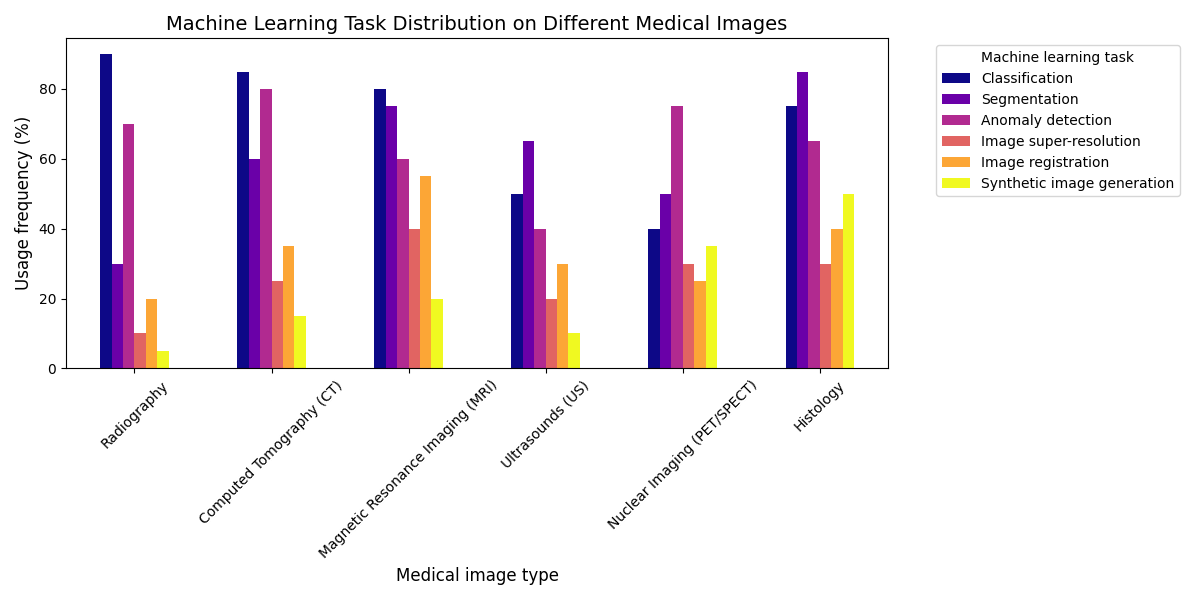
\includegraphics[width=0.9\textwidth]{Cap1/Figures/comparative-tasks-and-medical-image-types.png}
  \caption{Estimation of the popularity of tasks and medical image
    types based on
  recent literature review (count of referenced terms).}
  \label{fig:medical_image_analysis}
\end{figure}

For solving the different requirements of tasks in medical images, a
variety of computational techniques have been developed
\cite{Zhou2021}. Initially, these needs were covered with simple
morphological filters, which implied no training process or
elaborated optimization. However, as the complexity of the tasks
increased, the need for more sophisticated techniques arose, leading
to the application of advanced statistical tools and machine learning
algorithms like Support Vector Machines, Decision Trees, and SGD
Neural Networks \cite{Avanzo2024}. The coevolution of advances in medical image
acquisition, computational power (i.e. Moore's law) and
statistical/mathematical techniques have led to a convergence for
merging state of the art algorithms with medical imaging
\cite{Shalf2020}. Figure \ref{fig:medical-ai-timeline} shows a brief
timeline of coevolution between some conspicuous advances in
computational pattern recognition and its medical applications in
different scopes (besides medical imaging) \cite{Avanzo2024}.

\begin{figure}
  \centering
  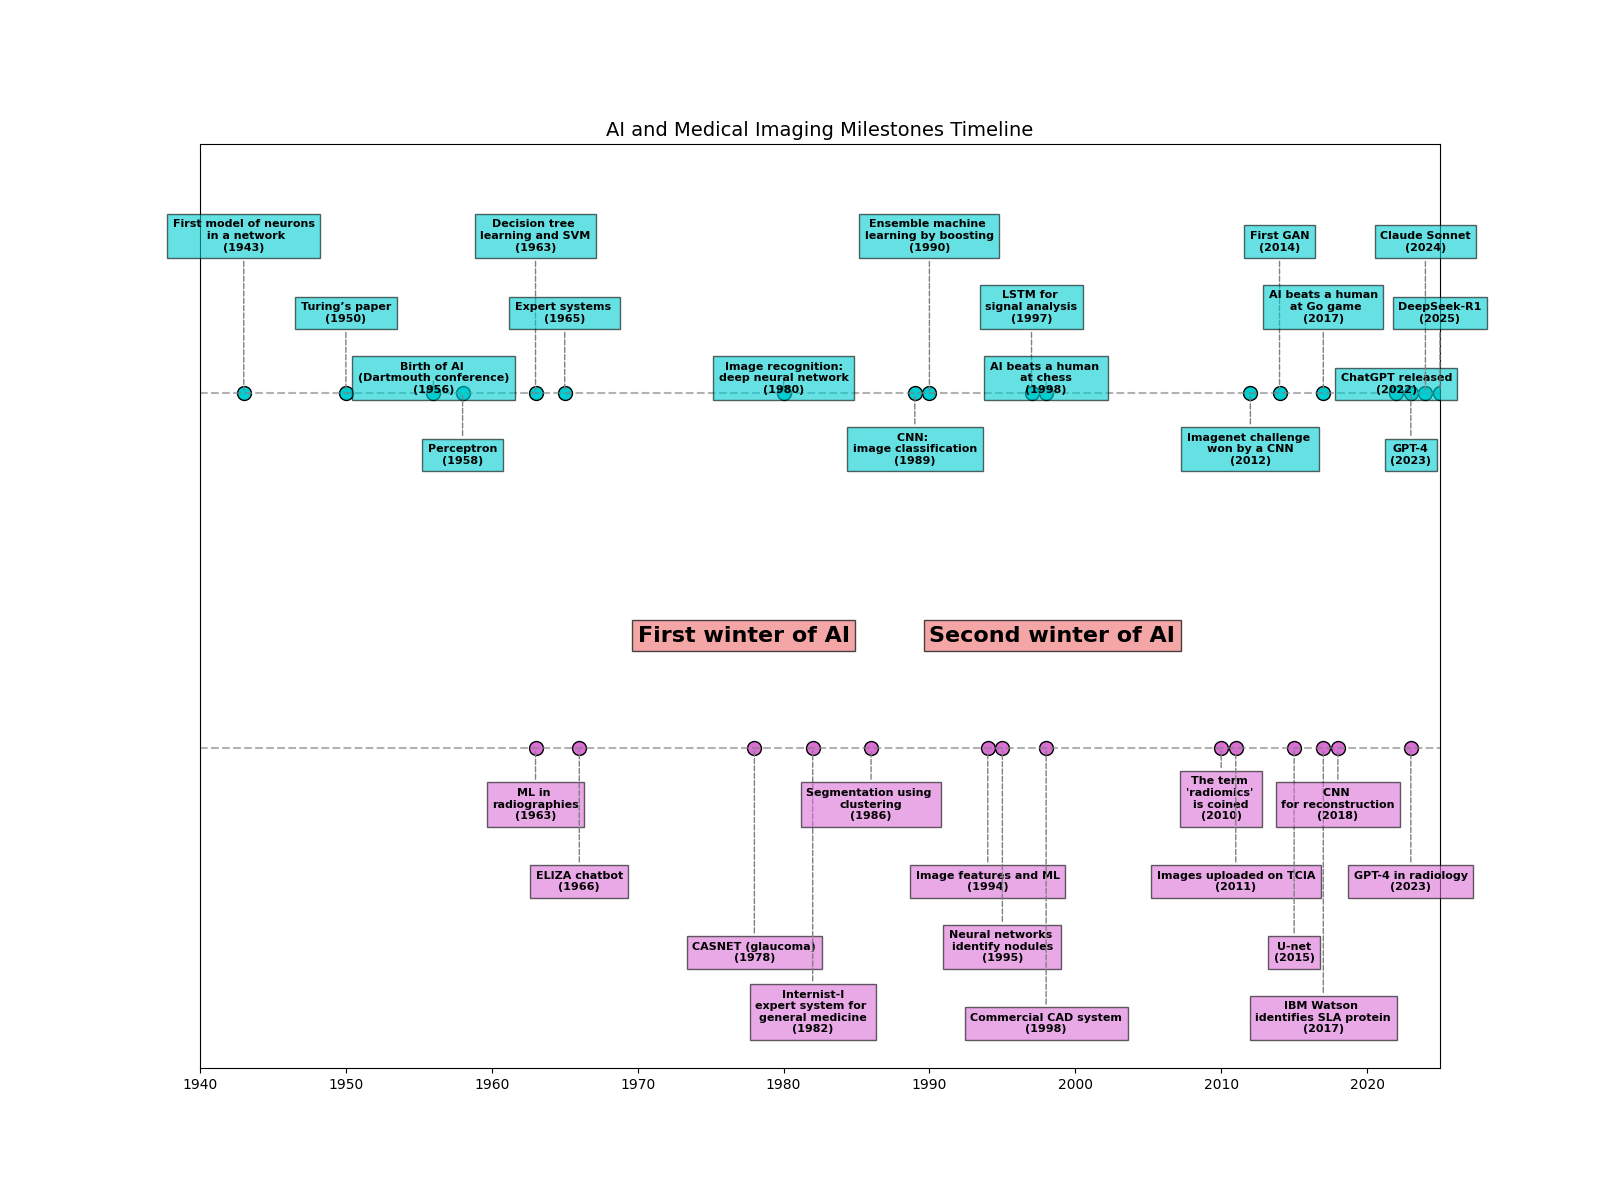
\includegraphics[trim={5cm 2cm 5cm
  0},width=0.9\textwidth]{Cap1/Figures/medical-ai-timeline.png}
  \caption{AI and machine learning in medical imaging brief timeline.}
  \label{fig:medical-ai-timeline}
\end{figure}

\gls{CNN} have been widely used in \gls{SS} tasks, as they have outperformed
traditional machine learning algorithms in this task for both medical
and non medical images \cite{XuYan2024} \cite{Sarvamangala2022}.
However, most \gls{CNN} architectures are deep, which imply
a necessity of a large amount of data to train them. This introduces
a problem since both the acquisition and annotation of medical images
are expensive and time-consuming processes. This is especially true
for \gls{ISS} tasks, as they require pixel-level annotations, which
is taxing in terms of cost, time and logistics involved
\cite{Bhalgat2018}. Other fashions face this problem through less expensive
annotation strategies like bounding boxes or anatomical landmarks for
being used in a semi-supervised strategy \cite{Shah2018}.

%% CHECKED

Many medical images datasets however, contain a high variability in
class sizes and variations in colors, which is specially noticeable
in histopathological images because of the usage of different
staining and other factors which can affect the color of the images
(see section \ref{sec:staining-techniques}).
This variability can lead to a significant loss of efficiency of
machine learning models when using a mixed supervision strategy, as
the model can be biased towards the most common classes or colors in
the dataset \cite{Shah2018}.

This is were other solutions arise to tackle the problem of the weak
image annotation while maintaining low costs. One of these solutions
is crowdsourcing strategy, which consists of having multiple annotators
labeling the same image, and then combining the labels to obtain a
consensus label \cite{LuEtAl2023}. This strategy can lead to a
labeling cost reduction when different levels of expertise are
combined, since the crowd may be composed of both experts and laymen,
being the latter less expensive to hire \cite{Lopez2023}.

Recently, diagnosis, prognosis and treatment of cancer have heavily
relied on histopathology, where tissue samples are obtained through biopsies or
surgical resections and critical information that helps
pathologists determine the presence and severity of malignancies
\cite{LopezEtAl2024}. The segmentation of histopathological images
enables precise identification of structures such as nuclei, glands, and tumors,
which are essential for assessing disease progression and treatment
response \cite{Rashmi2021}. Accurate segmentation is particularly
crucial in digital pathology, where whole-slide images (\gls{WSI})
are analyzed using AI-powered \gls{CAD} systems to support
clinical decision-making \cite{LopezEtAl2024}.

A major challenge in histopathological image segmentation arises from
the variability in annotations provided by different pathologists.
Unlike natural images, where object boundaries are often
well-defined, histological structures may have ambiguous borders,
leading to inconsistencies among annotators \cite{Lopez2023}. Because of this,
crowdsourcing labeling is one of the most popular approaches, as
illustrated in Figure \ref{fig:multiannotator_segmentation},
an example of how histopathological images are segmented by
multiple experts, showing some variations in label assignment
\footnote{obtained from a real world Triple Negative Breast
Cancer (TNBC) dataset published in \cite{Lopez2023}}. These
discrepancies highlight the need for models that can handle
annotation uncertainty effectively. Leveraging crowdsourcing
strategies and machine learning techniques that infer annotator
reliability can enhance segmentation performance while reducing costs.
\begin{figure}
  \centering
  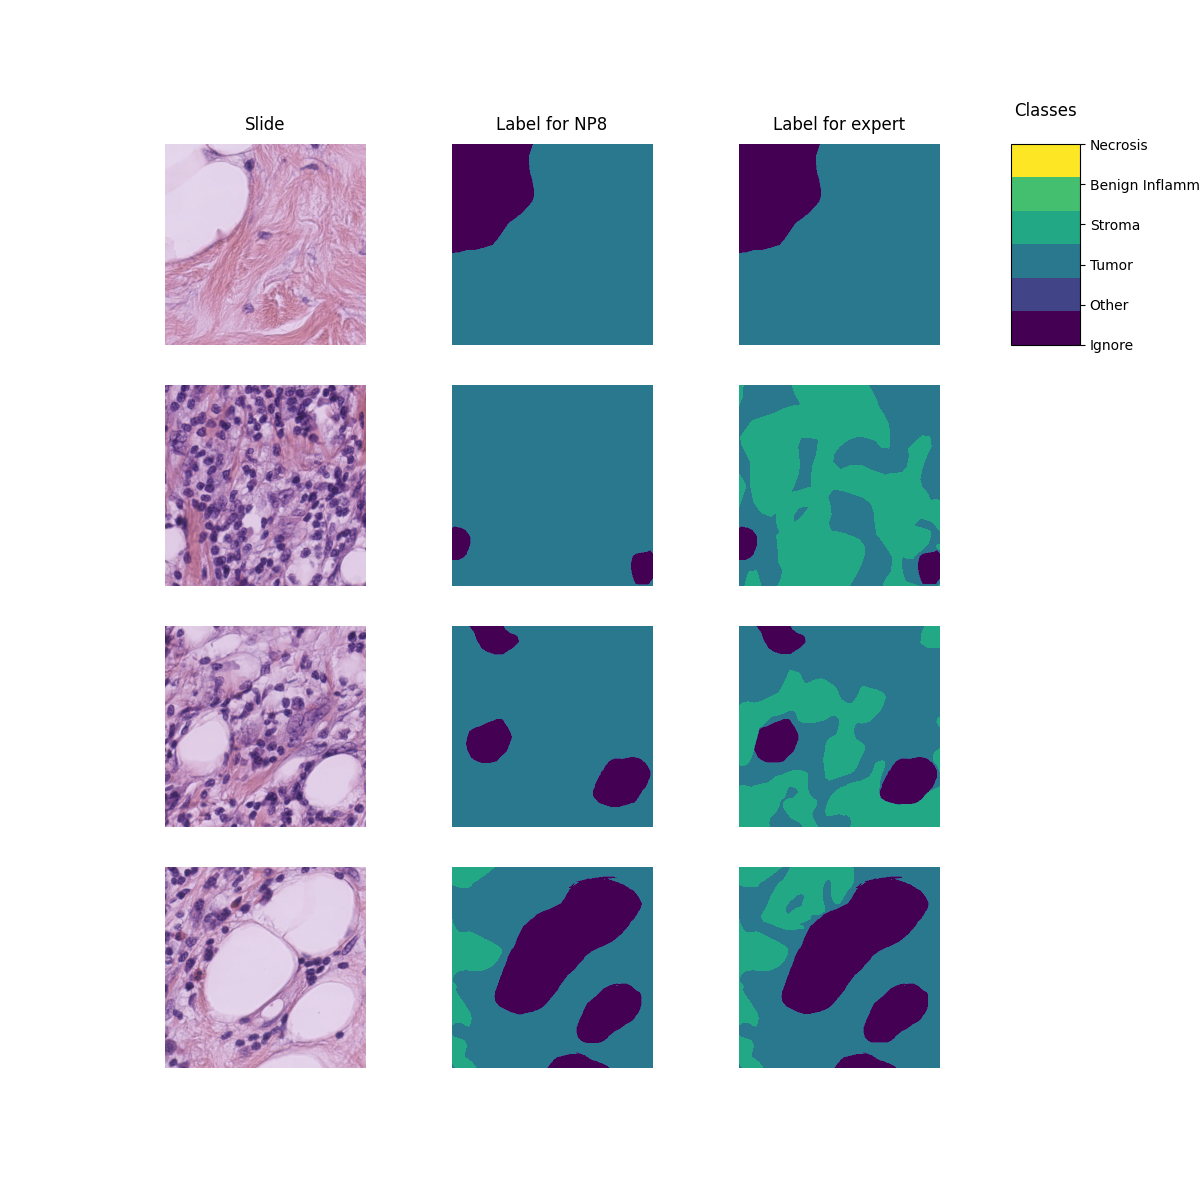
\includegraphics[width=0.9\textwidth]{Cap1/Figures/multiannotator-segmentation.png}
  \caption{Example of a histopathological image segmented by multiple
  annotators, illustrating variations in label assignment.}
  \label{fig:multiannotator_segmentation}
\end{figure}
\section{Problem Statement}\label{sec:state_of_art}

% ==============================
% Problem Statement Chapter
% ==============================

% Highlight the issue of inter-observer variability and the need for
% robust models that can learn from inconsistent labels.

Throughout the development of medical technology and \gls{CAD}, the
task of \gls{ISS} has become a crucial step in delivering precise diagnosis
and treatment planning \cite{Giri_Bhatia_2024}. Particularly, in the
area of histopathological studies, the usage of Whole Slide Images
(\gls{WSI}) is rather common since this method delivers high quality
imaging and allows for the diagnosis of diseases like cancer
\cite{YujiaEtAl2024}.

\gls{ISS} task consists of assigning a label to each pixel
in an image according to the object it belongs to. Accurate
segmentation is essential for the development of \gls{CAD} systems,
as it allows the identification of regions of interest (\gls{ROI}) in
the images, which can be used to detect and classify diseases and
hence, treatment planning \cite{Sarvamangala2022}. However, modern computational
solutions for \gls{ISS} tasks involve the use of deep learning, which
mostly rely large amounts of labeled data to train the models
on supervised learning techniques. This means that the model is trained on
a dataset with ground-truth labels, which are assumed to be correct
and consistent across all samples. In practice, this assumption is
often violated due to the high technical complexity of labeling these
segments \footnote{compared to a more trivial task like image classification
on ordinary an well known classes like MNIST}.

% The Multiple-Labelers Challenge
% Detail how medical images often require annotations from multiple
% experts with varying levels of expertise.
% Discuss common issues such as random errors (accidental mistakes)
% and expertise errors (systematic biases due to limited knowledge).
% Reference existing approaches that either require ground-truth
% labels or additional supervision to model labeler performance explicitly.

The process of labeling medical images is often managed with the help of
specialized software tools that allow the annotators to draw the
regions, delivering an standard format for the labeled
masks \cite{Habis2024}.
Despite the help of these tools, the labeling process in \gls{WSI} can have high
costs, as it requires long hours of work from specialized personnel.
Because of cost constraints in many medical institutions, the labeling processes
is often done by multiple labelers with varying levels of expertise, equalizing
the cost of the labeling process. However, this strategy can lead to
inconsistent labels, as the consensus between the labelers may not be
exact due to the diversity in depth of knowledge and experience of
the labelers \cite{XuYan2024}.
These inconsistencies are mostly represented in the subsections
\ref{subsec:expertise_levels} and \ref{subsec:technical_constraints}.

\subsection{Variability in Expertise Levels}\label{subsec:expertise_levels}

One of the primary sources of inter-observer variability in medical
image segmentation is the difference in expertise levels among
annotators \cite{Lopez2023}. Experienced radiologists and
pathologists tend to produce highly precise annotations, whereas
novice labelers may introduce systematic biases due to their limited
familiarity with subtle image features. Studies have demonstrated
that annotation accuracy \textit{tends} to improve with experience, yet medical
institutions often rely on a mix of annotators to manage costs and
workload distribution \cite{LuEtAl2023}.

The training background of annotators and institutional guidelines
play a crucial role in shaping labeling practices. Different medical
schools and hospitals may adopt distinct segmentation protocols,
leading to inconsistencies when datasets are combined from multiple
sources \cite{Lopez2023}. For example, some institutions may emphasize
conservative delineation of tumor boundaries, while others adopt a
more inclusive approach. Such variations contribute to systematic
biases in medical image datasets \cite{BanerjeeEtAl2025}.

Medical images frequently contain structures with ambiguous
boundaries, making segmentation inherently subjective. For instance,
tumor margins in histopathological slides may not have well-defined
edges, leading to variations in how different annotators delineate
the regions of interest \cite{Carmo2025}. These discrepancies arise not only
from technical expertise but also from differences in perception and
interpretation.

\subsection{Technical Constraints and Image
Quality}\label{subsec:technical_constraints}

Technical constraints in medical imaging, such as resolution
differences, noise levels, and contrast variations, can significantly
impact segmentation accuracy. Lower-resolution images may obscure
fine structures, leading to inconsistencies in boundary delineation
\cite{ZhouEtAl2024}.

When combined with long sessions, bad images might
also increase the cognitive load of the annotators, leading to
fatigue and reduced precision in labeling \cite{KimYujinAndLee2024}.
This is particularly relevant in histopathological studies, where the
staining process and tissue preparation can introduce color
variations and artifacts that affect image quality, even if the same scanning
equipment is used \cite{Karthikeyan2023}.

\begin{figure}
  \centering
  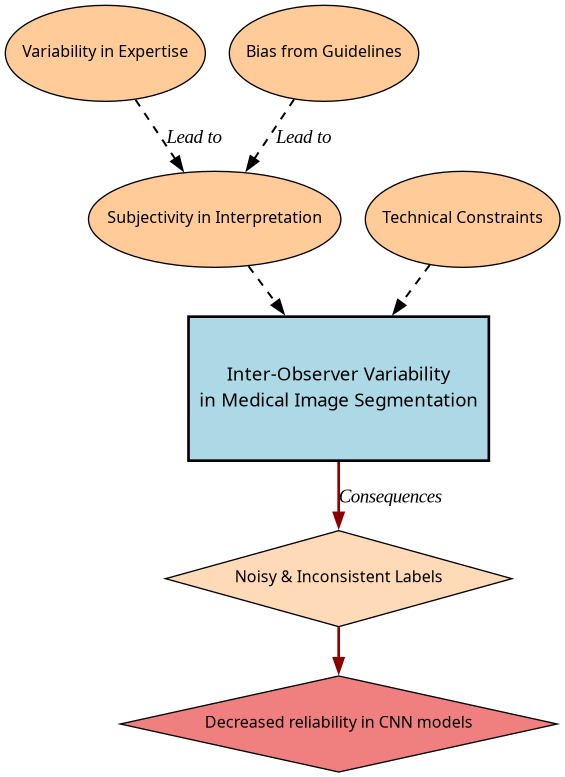
\includegraphics[width=0.7\textwidth]{Cap1/Figures/problem_statement_diagram.png}
  \caption{Summary diagram for problem Statement}
  \label{fig:problem_statement_diagram}
\end{figure}

\subsection{Research Question}

Given the challenges posed by inconsistent labels in medical image
segmentation, this work aims to address the following research
question:

\researchquestion{How can we develop a learning approach for
  \gls{ISS} tasks in medical images that can adapt to inconsistent
  labels without requiring explicit supervision of labeler
  performance, while addressing challenges related to variability in
  expertise levels and technical constraints, and maintaining
interpretability, generalization, and computational efficiency?}
\section{Literature review}\label{sec:state_of_art}

Certainly, in general \gls{ML} classification tasks \footnote{In this
  work, image segmentation is considered as a particular case of classification
in which target classes are assigned pixel-wise.} where multiple
annotators are involved, \gls{MV} is by far the simplest
possible approach to implement. This concept was born multiple times
and divergently in multiple fields, but it was described as relevant
for \gls{ML} and pattern recognition labeling for classification in
\cite{LamAndSuen1997}, in which the approach is exposed as simple,
yet powerful. The authors describe the \gls{MV} as a method that can
be used to improve the accuracy of classification tasks by combining
the labels of multiple annotators. The method is based on the
assumption that the majority vote of the annotators is more likely to
be correct than the vote of a single annotator. The authors also
describe the method as a straightforward way to improve the accuracy
of classification tasks without the need for complex algorithms or
additional data. The authors also prove this method to deliver very
similar results to more complicated approaches (Bayesian, logistic
regression, fuzzy integral, and neural network) in the
particular task of \gls{OCR}. Despite its simplicity, modern
solutions for delivering accurate medical image segmentation models
still rely on Majority Voting at some stage, like \cite{Elnakib2020},
which uses a majority voting strategy for delivering a final output
based on the labels of multiple models (VGG16-Segnet, Resnet-18 and
Alexnet) in \gls{CT} images for Liver Tumor Segmentation, or
\cite{Lopez2023}, which uses \gls{MV} for combining noisy annotations
as an additional annotator to be included in the deep learning solution.
Majority voting as a technique for setting a pseudo ground truth label
is a powerful approach for its simplicity in many use cases in which
the target to be labeled is not tied to an expertise related task,
otherwise, the assumption of equal expertise among the labelers can
be a source of bias in the final label, which is not desirable in the
case of highly technical annotations like medical images.
In subsection \ref{subsec:expertise_levels_lit_review}, we will be
reviewing literature which no longer assumes the naive approach of
equal expertise among labelers and face the challenge of learning
from inconsistent labels.

\subsection{Facing annotation variability in medical
images}\label{subsec:expertise_levels_lit_review}

Learning from crowds approaches in general face the challenge of
not having a ground truth label and hence, an intrinsic difficulty in
measuring the real reliability of the labelers annotations. Some
approaches assume beforehand a certain level of expertise for each
labeler based on experience as an input, like in
\cite{TianEtZhu2015}, which introduce the concept of max margin
majority voting, using the reliability vector as weights for the
weights for the binary and multiclass classifier. The crowdsourcing
margin is the minimal difference between the aggregated score of the
potential true label and the scores for other alternative labels.
Accordingly, the annotators' reliability is estimated as generating
the largest margin between the potential true labels and other
alternatives. The problem introduced in this approach is assuming an
stationary reliability per expert across the whole input space, which
is imprecise since annotators performance may change between
different tasks or even between different regions of the same image.

% REVIEW
\subsubsection{STAPLE Mechanism}

The \gls{STAPLE} algorithm, introduced in \cite{WarfieldEtAl2004}
is a probabilistic framework that estimates a hidden true
segmentation from multiple segmentations provided by
different raters. It also estimates the reliability of each rater by
computing their sensitivity and specificity.

The \gls{STAPLE} algorithm's goal is to maximize the log likelihood function:

\begin{equation}\label{eq:staple_likelilhood}
  (\mathbf{\hat{p}}, \mathbf{\hat{q}}) = \arg\max_{\mathbf{p}, \mathbf{q}} \ln
  f(\mathbf{D},
  \mathbf{T} \mid \mathbf{p}, \mathbf{q}).
\end{equation}

Where $\mathbf{D}$ is the set of segmentations provided by the raters,
$\mathbf{T}$ is the hidden true segmentation, $p$ is the sensitivity
and $q$ is the specificity of the raters.

This is achieved by using the Expectation-Maximization algorithm to
maximize the log likelihood function in equation, which is done iteratively
with step computations:

\begin{equation}
  \begin{split}
    (p_j^{(k)}, q_j^{(k)}) = \arg\max_{p_j, q_j} \sum_{i:D_{ij}=1}
    W_i^{(k-1)} \ln p_j \\
    &+ \sum_{i:D_{ij}=1} \left(1 - W_i^{(k-1)}\right) \ln (1 - q_j) \\
    &+ \sum_{i:D_{ij}=0} W_i^{(k-1)} \ln (1 - p_j) \\
    &+ \sum_{i:D_{ij}=0} \left(1 - W_i^{(k-1)}\right) \ln q_j.
  \end{split}
\end{equation}

The capacity of STAPLE to accurately estimate the true segmentation,
even in the presence of a majority of raters generating correlated
errors, was demonstrated, which makes it theoretically a strong
choice for setting a ground-truth in binary or multiclass medical
\gls{ISS} tasks.

The popularity and performance of \gls{STAPLE} has led to its
usage in modern applications medical image, 3d spatial images due to
its assumption of decision space being based on voxel-wise decisions,
like the authors in \cite{GrefveEtAl2024} which applied the algorithm
on \gls{PET} images. Other authors still rely heavily on STAPLE for
setting a ground truth consensus for histopathological images, like
\cite{QiuEtAl2022}.

However, the \gls{STAPLE} algorithm has some limitations. It
assumes independent rater errors, which may not hold in practice,
leading to biased estimates. STAPLE is also sensitive to low-quality
annotations, potentially degrading final segmentations if the weights
are not initialized correctly. The algorithm tends to over-smooth
results, blurring fine details, and struggles with multi-class
segmentation. Computationally, it is expensive due to its iterative
EM approach. Additionally, STAPLE cannot correct systematic biases in
annotations and depends on initial estimates, impacting accuracy.
Lastly, the estimated performance levels lack interpretability,
making it difficult to assess annotator reliability effectively.

Finally, this work contemplates \gls{STAPLE} as useful for ground
truth estimation given the existence of multiple labelers for an
input \gls{WSI}, but not that useful for providing annotations of structures on
new and unlabeled images, hence being a good support for other methods.

\subsubsection{Chained Gaussian Processes}

Other works like \cite{GilGonzalesEtAl2025} proposed a novel approach

\subsection{Strategies for handling low-quality images}

The problem of low-quality images and noisy annotations has been
tackled with various strategies. One such approach is the use of deep
learning models that incorporate loss functions designed to mitigate
the effects of unreliable labels. Traditional methods such as
Majority Voting (MV) or Expectation-Maximization (EM) have been
widely used for aggregating multiple annotators' inputs. However,
they assume a homogeneous reliability of annotators, which may not
hold in real-world scenarios.

A more recent approach was proposed by \cite{TrianaEtAl2023},
introducing a Generalized Cross-Entropy-based Chained Deep Learning
(GCECDL) framework. This method addresses the limitations of
traditional label aggregation techniques by modeling each annotator's
reliability as a function of the input data. The approach effectively
mitigates the impact of noisy labels by using a noise-robust loss
function, balancing Mean Absolute Error (MAE) and Categorical
Cross-Entropy (CE). Unlike prior approaches, GCECDL accounts for the
dependencies among annotators while encoding their non-stationary
behavior across different image regions. Their experiments on
multiple datasets demonstrated superior predictive performance
compared to state-of-the-art methods, particularly in cases where
annotations were highly inconsistent.

This strategy is especially relevant for handling low-quality medical
images, where expert annotations may be inconsistent, and traditional
consensus-based approaches fail to account for varying expertise
levels. By leveraging deep learning with robust noise-handling loss
functions, the reliability of segmentation models can be significantly improved.


\section{Aims}\label{sec:objectives}

With the mentioned considerations in section \ref{sec:state_of_art}
in mind, this work proposes a novel approach for \gls{ISS} tasks in
medical images, which aims to train a model whose learning approach
is adaptive to the labeler performance. This is done by introducing a
loss function capable of inferring the best possible segmentation
without needing separate inputs about the labeler performance. This
loss function is designed to implicitly weigh the labelers based on
their performance, with the presence of an intermediate reliability
map allowing the model to learn from the most reliable labelers and
ignore the noisy labels. This approach differs from existing
\gls{CNN}-based segmentation models, as it does not require explicit
supervision of the labeler performance, making it more generalizable
and adaptable to different datasets and labelers.
\subsection{General Aim}

The main purpose of this work is to develop a novel approach for
\gls{ISS} tasks in medical images, which can adaptively infer the best
possible segmentation without needing separate inputs about the
labeler performance. This approach is expected to outperform the
segmentation performance of other state of the art approaches,
eliminate the need for explicit labeler supervision, and enhance
automation in medical image analysis.

%----------------------------------------------------------------------
\subsection{Specific Aims}

\begin{itemize}

  \item To develop a novel loss function for \gls{ISS} tasks in
    medical images, capable of inferring the best possible
    segmentation without needing separate inputs about the labeler
    performance.

  \item Introducing a tensor map which codifies the reliability of
    each labeler, allowing the model to implicitly weigh the labelers
    based on their performance across the mask and classes space.

  \item To develop and test a deep learning model for \gls{ISS} tasks
    in medical images, which can learn from inconsistent labels and
    improve the segmentation performance compared to other solutions
    in state of the art.

\end{itemize}


\clearpage
\section{Outline and Contributions}

As an output of this work, some contributions were made to the field of
\gls{ISS} in medical images. The main contributions are:

\begin{itemize}
  \item A python package for using the proposed loss function in
    \gls{CNN} models for \gls{ISS} tasks in medical images.
    \footnote{https://pypi.org/project/seg\_tgce/}
  \item Datasets mapping as lazy loaders for the proposed loss
    function.
    \footnote{https://seg-tgce.readthedocs.io/en/latest/experiments.html}
  \item A public Github repository with the code used in this work.
    \footnote{https://github.com/blotero/seg\_tgce}
\end{itemize}

\glsreset{SS}

\chapter{Conceptual preliminaries}\label{cap:conceptual_preliminaries}

\section{Modern concept of digital image}

A digital image is a numerical representation of a visual scene,
captured through various imaging devices and stored in a computer.
From a mathematical perspective, a digital image can be represented
as a function $f(x,y)$ that maps spatial coordinates $(x,y)$ to
intensity values. In the discrete domain, this function is sampled at
regular intervals, creating a matrix of values known as pixels
(picture elements).

\subsection{Types of digital images}

\subsubsection{Grayscale images}
Grayscale images are the simplest form of digital images, where each
pixel represents a single intensity value. Mathematically, a
grayscale image can be represented as a 2D matrix $I$ of size $M
\times N$, where each element $I(i,j)$ represents the intensity at
position $(i,j)$. The intensity values typically range from 0 (black)
to 255 (white) in 8-bit images, or from 0 to 65535 in 16-bit images.

\subsubsection{Color images}
Color images extend the grayscale concept by representing each pixel
with multiple channels, typically Red, Green, and Blue (RGB). A color
image can be represented as a 3D matrix $I$ of size $M \times N
\times 3$, where $I(i,j,k)$ represents the intensity of the $k$-th
color channel at position $(i,j)$. Other color spaces like HSV (Hue,
Saturation, Value) or CMYK (Cyan, Magenta, Yellow, Key) are also
commonly used in different applications.

\subsubsection{Multispectral images}
Multispectral images capture information across multiple wavelength
bands beyond the visible spectrum. These images can be represented as
a 3D matrix $I$ of size $M \times N \times B$, where $B$ is the
number of spectral bands. Each band $I(i,j,b)$ represents the
intensity at position $(i,j)$ for the $b$-th spectral band. This
representation is particularly useful in medical imaging, remote
sensing, and scientific applications.

\subsubsection{3D images and volumetric data}
Three-dimensional images extend the concept of pixels to voxels
(volume elements). A 3D image can be represented as a 3D matrix $V$
of size $M \times N \times D$, where $D$ represents the depth
dimension. Each voxel $V(i,j,k)$ represents the intensity at position
$(i,j,k)$ in the 3D space. This representation is fundamental in
medical imaging (CT, MRI), scientific visualization, and computer graphics.

\subsection{Mathematical representations}

The mathematical foundation of digital images relies on several key concepts:

\begin{itemize}
  \item \textbf{Sampling}: The process of converting a continuous
    image into a discrete representation. According to the
    Nyquist-Shannon sampling theorem, the sampling frequency must be
    at least twice the highest frequency present in the image to avoid aliasing.

  \item \textbf{Quantization}: The process of converting continuous
    intensity values into discrete levels. The number of quantization
    levels determines the image's bit depth and affects its quality
    and storage requirements.

  \item \textbf{Resolution}: The number of pixels per unit length in
    an image, typically measured in pixels per inch (PPI) or dots per
    inch (DPI).

  \item \textbf{Dynamic range}: The ratio between the maximum and
    minimum measurable light intensities in an image, often expressed
    in decibels (dB).
\end{itemize}

The mathematical representation of a digital image can be expressed as:

\begin{equation}
  I(x,y) = \sum_{i=0}^{M-1} \sum_{j=0}^{N-1} f(i,j) \cdot \delta(x-i, y-j)
\end{equation}

where $I(x,y)$ is the digital image, $f(i,j)$ represents the
intensity values, and $\delta(x-i, y-j)$ is the Kronecker delta function.

For color images, the representation extends to:

\begin{equation}
  I(x,y) =
  \begin{bmatrix}
    I_R(x,y) \\
    I_G(x,y) \\
    I_B(x,y)
  \end{bmatrix}
\end{equation}

where $I_R$, $I_G$, and $I_B$ represent the red, green, and blue
channels respectively.

\section{Digital histopathological images}

\glsreset{WSI}
\glsreset{ROI}

Digital histopathology represents a significant advancement in
medical imaging, where traditional glass slides containing tissue
samples are digitized using specialized scanning devices. This
transformation has revolutionized the field of pathology by enabling
remote diagnosis, computer-aided analysis, and digital archiving of
tissue samples \cite{AmgadEtAl2019}. This process has evolved
significantly over the past few decades, as shown in Figure
\ref{fig:histology_evolution}.

\begin{figure}[h]
  \centering
  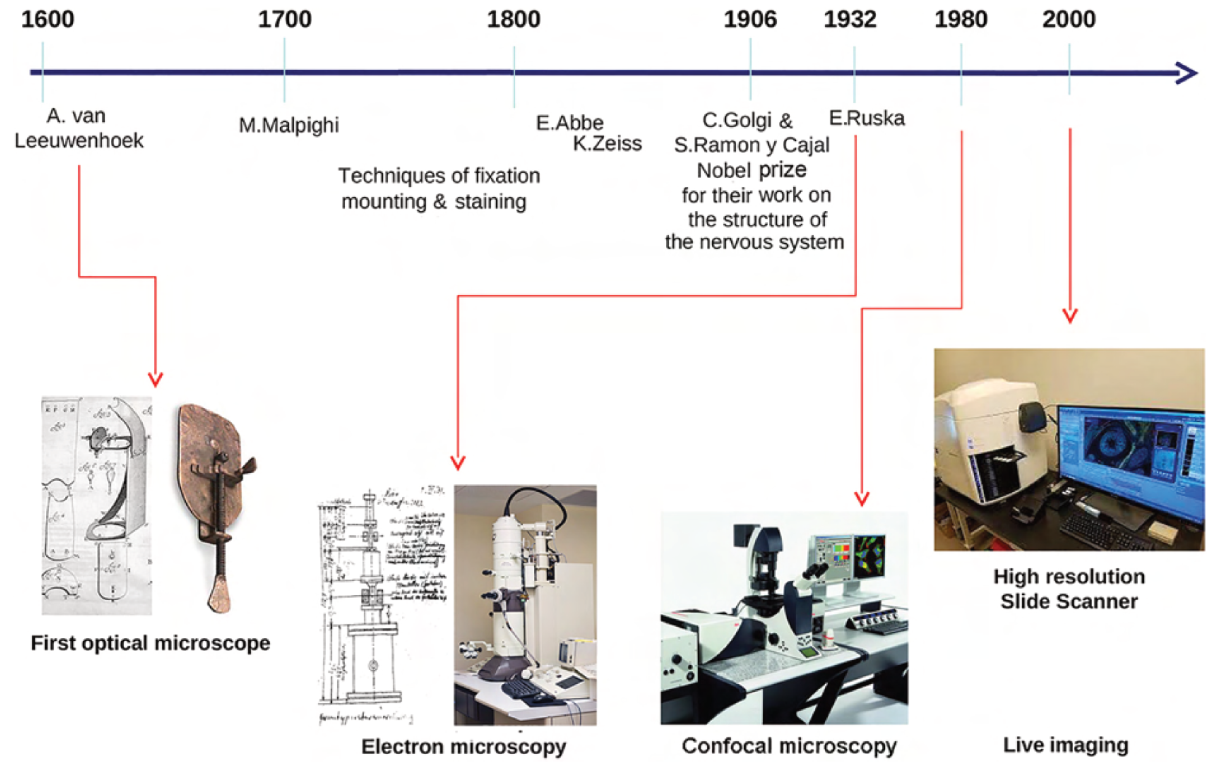
\includegraphics[width=0.65\textwidth]{Cap2/Figures/histology_evolution.png}
  \caption{Histology evolution timeline. (Image from \cite{MazzariniEtAl2021}).}
  \label{fig:histology_evolution}
\end{figure}

\subsection{Whole Slide Imaging (WSI)}

\gls{WSI} is the process of digitizing entire glass
slides at high resolution, creating a digital representation that can
be viewed, analyzed, and shared electronically. Modern \gls{WSI} scanners
use sophisticated optical systems that capture multiple fields of
view at high magnification, which are then stitched together to
create a seamless digital image \cite{DingyiEtAl2025}. These systems incorporate
high-resolution objectives with magnifications ranging from 20x to
40x, precise motorized stages for accurate slide positioning,
automated focus systems to maintain image quality, and high-quality
cameras equipped with large sensor arrays. The resulting digital
slides can reach sizes of several gigabytes, containing billions of
pixels that capture the microscopic details of tissue samples
\cite{DingyiEtAl2025}. Figure \ref{fig:wsi} shows a whole slide
imaging system by Omnyx for slide digitization and a comprehensive
digital pathology interface from Omnyx designed to streamline
pathologists' diagnostic workflow \cite{FarahaniEtAl2015}.

\begin{figure}[h]
  \centering
  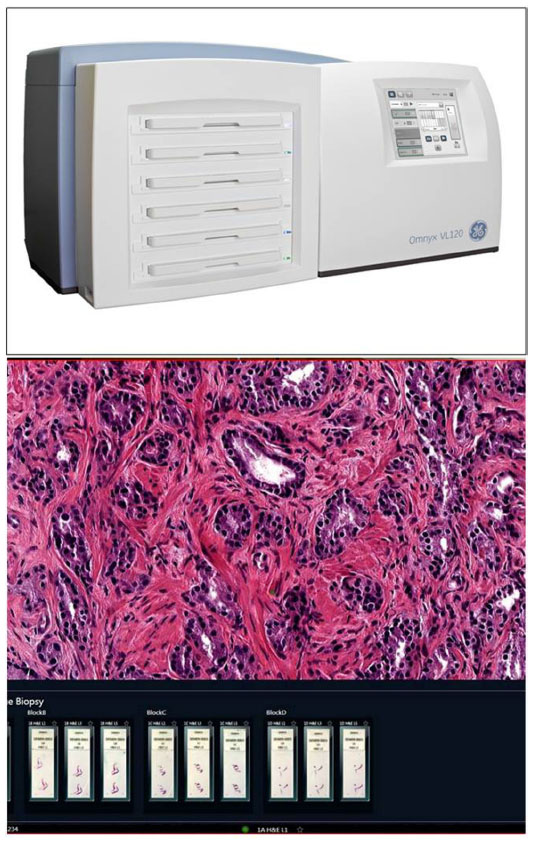
\includegraphics[width=0.5\textwidth]{Cap2/Figures/hist_scanner.jpg}
  \caption{(Above) Whole slide imaging system by Omnyx for slide
    digitization. (Below) Comprehensive digital pathology interface
    from Omnyx designed to streamline pathologists' diagnostic
  workflow. (From \cite{FarahaniEtAl2015}).}
  \label{fig:wsi}
\end{figure}

\subsection{Regions of Interest (ROI)}

In digital histopathology, \glspl{ROI} are specific areas within a
whole slide image that contain diagnostically relevant information.
These regions can be manually annotated by pathologists,
automatically detected using computer vision algorithms, or defined
based on specific tissue characteristics or abnormalities. The
importance of \glspl{ROI} lies in their ability to focus
computational analysis on relevant areas, reduce computational
complexity in automated systems, facilitate targeted diagnosis and
research, and enable efficient storage and transmission of critical information.

\subsection{Staining Techniques}\label{sec:staining_techniques}

Histopathological analysis relies heavily on various staining
techniques to enhance the visibility of different tissue components
and cellular structures. The choice of staining method depends on the
specific diagnostic requirements and the type of tissue being examined.

\subsubsection{Hematoxylin and Eosin (H\&E)}

Hematoxylin and Eosin (H\&E) staining is the most widely used
technique in histopathology, particularly in breast cancer diagnosis
\cite{PanEtAl2021}. This staining method provides essential visualization
through two components: hematoxylin, which stains cell nuclei
blue/purple to highlight nuclear morphology, and eosin, which stains
cytoplasm and extracellular matrix pink/red to reveal tissue architecture.

The popularity of H\&E staining in breast cancer histopathology stems
from its ability to clearly visualize tumor architecture and growth
patterns, distinguish between different types of breast cancer,
identify important diagnostic features like nuclear pleomorphism, and
assess tumor grade and stage. Beyond breast cancer, H\&E staining
finds extensive application across various medical specialties
including general pathology, dermatology, gastroenterology,
neurology, and oncology.

\subsubsection{Special Stains}

In addition to H\&E, various special stains are used for specific
diagnostic purposes. Immunohistochemistry (IHC) uses antibodies to
detect specific proteins, playing a crucial role in subtyping breast
cancers. Key IHC stains include Estrogen Receptor (ER) staining for detecting
estrogen receptors, Progesterone Receptor (PGR) staining for assessing
progesterone receptor status, Human Epidermal Growth Factor Receptor 2
(HER2) staining for evaluating HER2 protein expression, and Ki67
staining for measuring cellular proliferation rates. These markers are
particularly crucial in breast cancer diagnosis and treatment planning,
as they help determine the molecular subtype of the cancer and guide
personalized therapeutic approaches. Other specialized stains include
Periodic Acid-Schiff (PAS) for highlighting carbohydrates and basement
membranes, Masson's Trichrome for distinguishing between collagen and
muscle fibers, and silver stains for detecting microorganisms and
nerve fibers. These specialized staining techniques complement H\&E
by providing additional diagnostic information that is crucial for
accurate diagnosis and treatment planning \cite{WeitzEtAl2023}.
Examples of these staining techniques are shown in Figure
\ref{fig:weitz_dataset_overview}.


\section{Deep learning fundamentals}

Deep learning has emerged as a powerful subset of machine learning,
revolutionizing the field of artificial intelligence. Its roots can
be traced back to the early development of artificial neural networks
in the 1940s and 1950s, with significant milestones including the
perceptron in 1958 and the backpropagation algorithm in the 1980s.
However, it wasn't until the early 21st century, with the advent of
more powerful computational resources and the availability of large
datasets, that deep learning truly began to flourish.

\subsection{Learning Paradigms}

Deep learning systems can be categorized into three main learning paradigms.
The most common approach is supervised learning, where models learn from
labeled data by mapping inputs to known outputs. This paradigm requires a
large amount of labeled training data, which can be expensive and
time-consuming to acquire. Semi-supervised learning offers a hybrid
approach that leverages both labeled and unlabeled data, proving
particularly useful when labeled data is scarce but unlabeled data is
abundant. Finally, unsupervised learning enables models to discover
patterns and structures from unlabeled data without explicit guidance,
making it valuable for tasks like clustering and dimensionality
reduction.

\subsection{Architecture and Training}

Deep learning architectures are characterized by their layered
structure, where each layer progressively extracts and transforms
features from the input data. The early layers typically focus on
low-level feature extraction, such as edges, textures, and basic
patterns in the case of image processing. As information flows through
the network, middle layers combine these basic features into more
complex representations. The final layers perform high-level reasoning
and make the ultimate predictions or classifications.

The training process relies heavily on the gradient descent
algorithm, which iteratively adjusts the model's parameters to
minimize a loss function. This loss function serves as a crucial
component of the learning process, quantifying how well the model's
predictions match the actual targets. By providing a measure of the
model's performance, the loss function guides the optimization process,
enabling the network to learn meaningful patterns from the training
data.

\subsection{Challenges and Solutions}

Despite their power, deep learning systems face several significant
challenges. One of the most prominent issues is overfitting, where
models may memorize training data instead of learning generalizable
patterns. This challenge is typically addressed through various
regularization techniques such as dropout, L1/L2 regularization, and
early stopping. Another critical challenge is the substantial data
requirements; deep learning models often need massive amounts of
training data to achieve good performance, which can be a limiting
factor in many applications. Additionally, the complex, layered nature
of deep learning models makes them difficult to interpret, often
referred to as "black boxes." This lack of transparency can be
particularly problematic in critical applications where understanding
the decision-making process is essential.

\subsection{Deep Learning Frameworks}

The development of powerful open-source frameworks has significantly
accelerated deep learning research and applications. TensorFlow,
developed by Google, provides a comprehensive ecosystem for building
and deploying machine learning models. PyTorch, created by Facebook's AI
Research lab, offers dynamic computation graphs and has become
particularly popular in research settings. Caffe, known for its speed and modularity, is widely used in computer vision applications.

These frameworks have democratized deep learning by providing
efficient implementations of common operations, automatic
differentiation for gradient computation, and GPU acceleration for
faster training. They also offer pre-trained models and transfer
learning capabilities, along with active communities for support and
knowledge sharing. The combination of these frameworks with modern
hardware has enabled researchers and practitioners to develop
increasingly sophisticated models, pushing the boundaries of what's
possible in artificial intelligence. As shown in
Figure~\ref{fig:dl_frameworks_trends}, which presents data from
Google Trends over the last five years (as of April 2025), TensorFlow
and PyTorch have emerged as the two most prominent frameworks in the
deep learning landscape.

\begin{figure}[h]
  \centering
  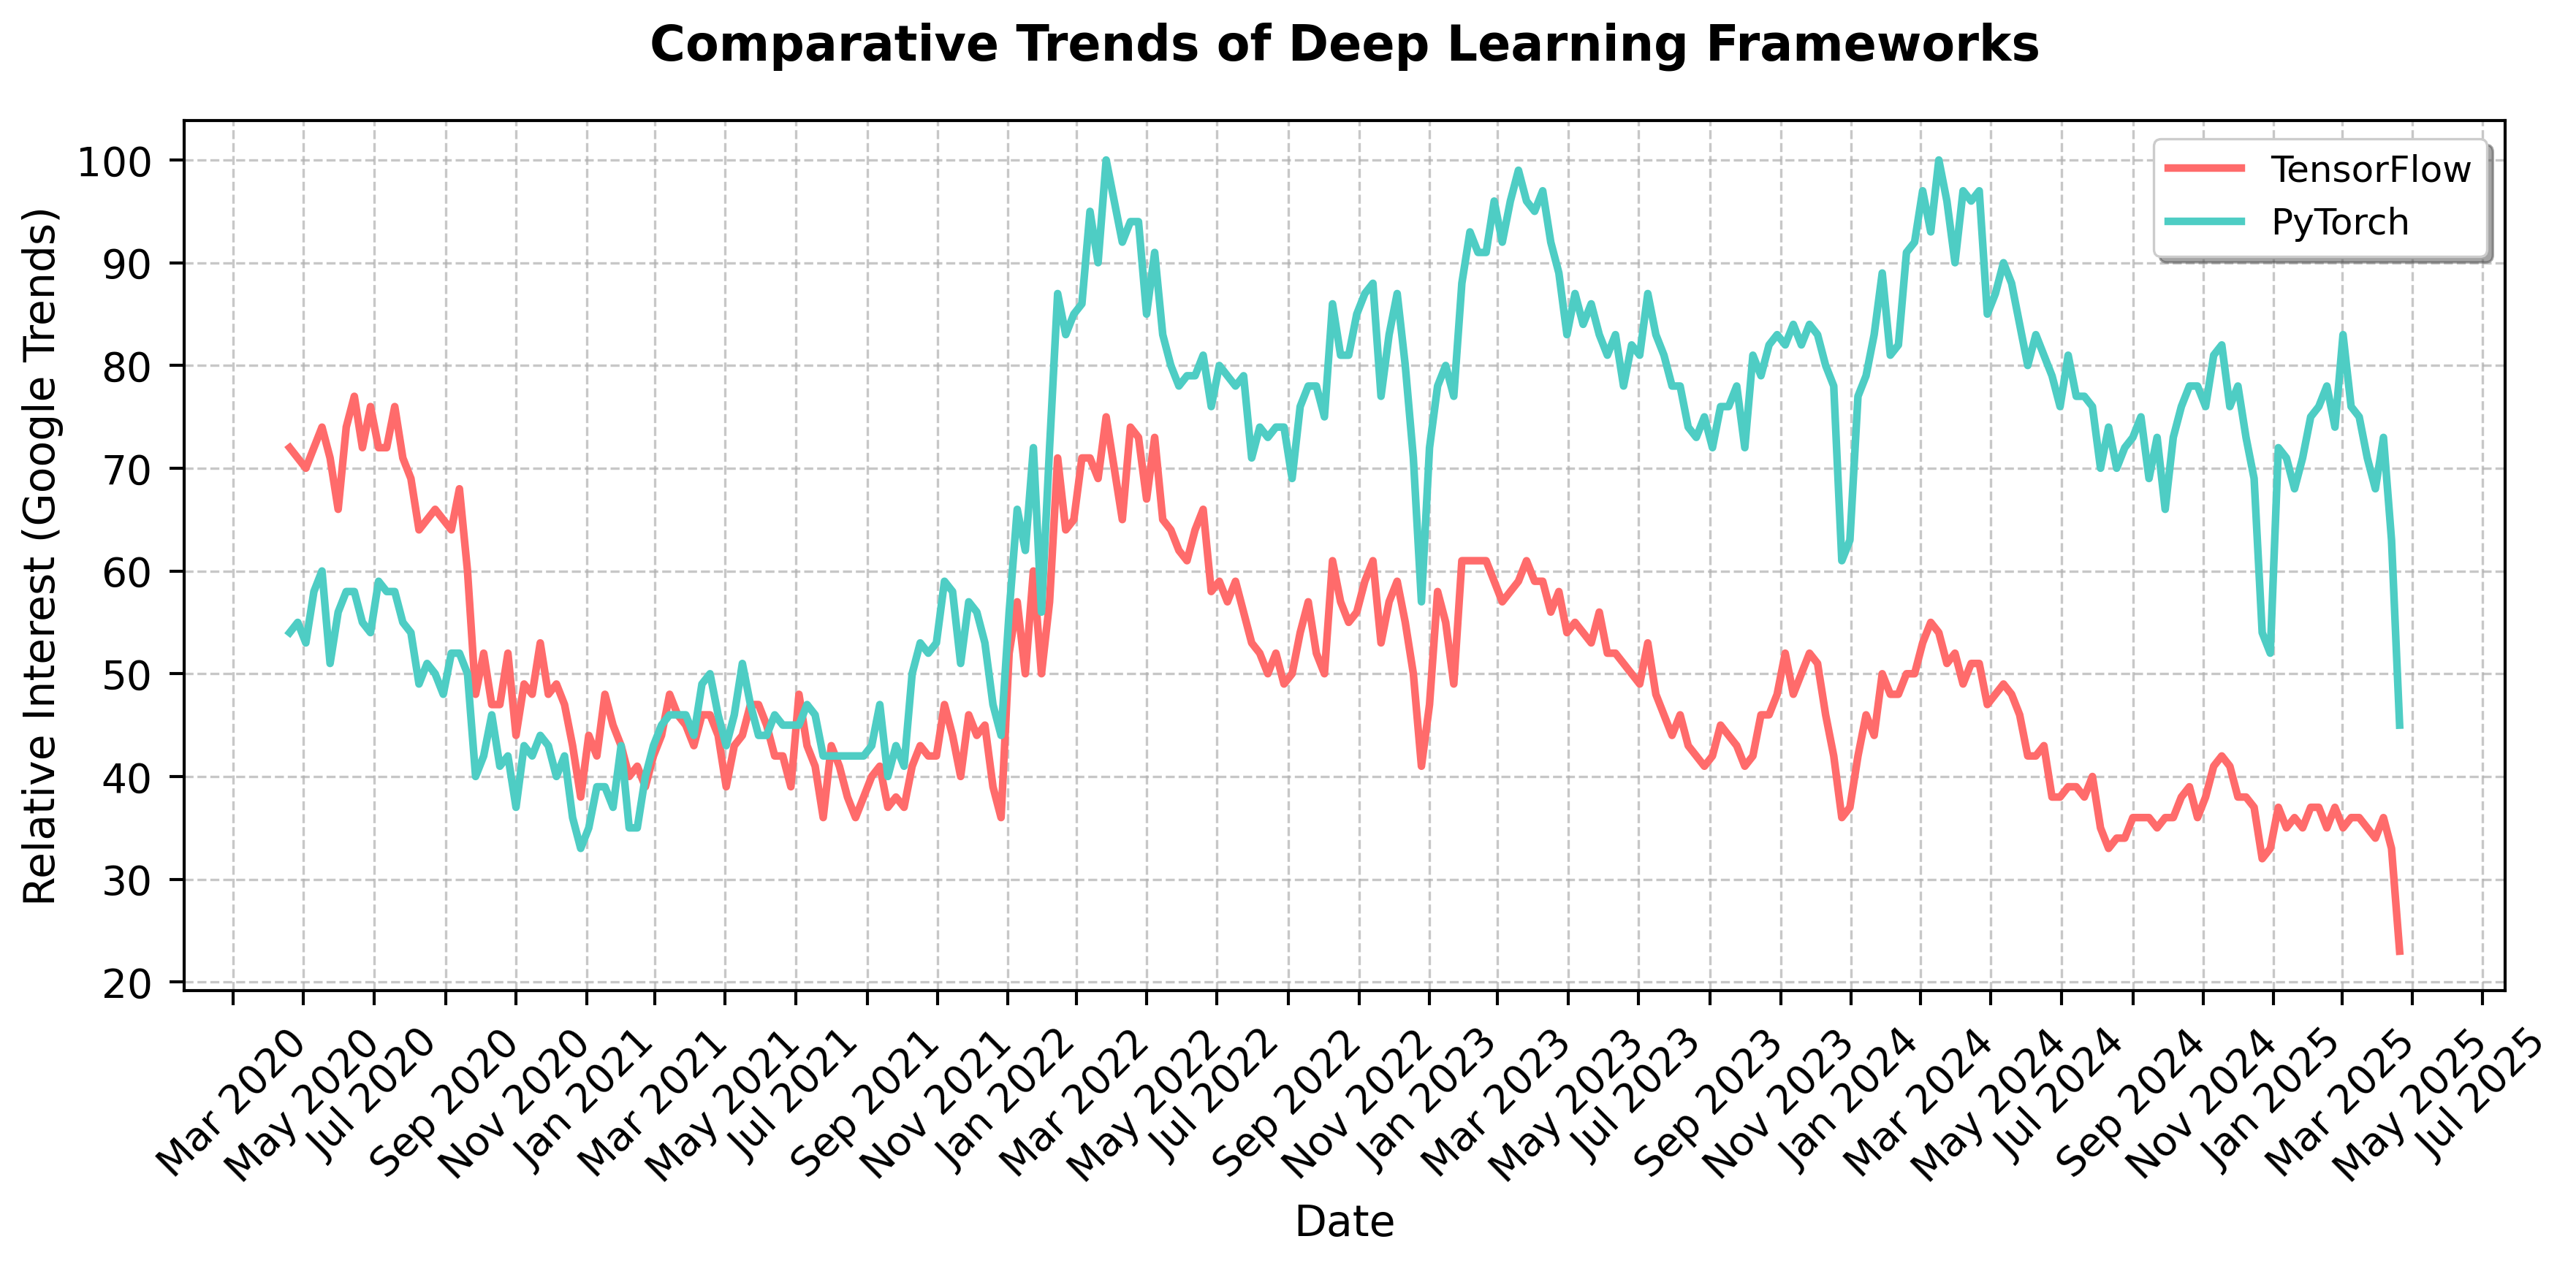
\includegraphics[width=0.8\textwidth]{Cap2/Figures/dl_frameworks_trends.png}
  \caption{Comparative Trends of the top two most popular Deep
  Learning Frameworks}
  \label{fig:dl_frameworks_trends}
\end{figure}


\section{Datasets and data sources}

Throughout the development of this work, multiple datasets were used
for evaluation of \gls{ISS} models. The common elements of all these datasets
are that they contain RGB images and are crowdsourced with multiple
labelers, where not necessarily all labeler label all images.

As it has been mentioned in Chapter \ref{ch:introduction}, the main goal of this
work is mainly focused on crowdsourced histopathology images semantic
segmentation, however, these datasets present the following challenges:

\begin{itemize}
  \item Distribution of segmentation labels is not uniform across the
    image, since some tissues and structures are more common than others.
  \item Visualization of performance of the models in debug time (like per epoch
    analysis) is not simple for non experts in the subject, which makes it
    hard to evaluate whether the model is overfitting or not at a glance.
\end{itemize}

For these reasons, multiple datasets were created in the pursuit of
an initial evaluation of performance of the models against more traditional
and familiar images before the focus on histopathology images. Once a
decent performance in metrics like Dice coefficient was achieved, the
focus was shifted to histopathology images and further tunings on the models
were performed if needed.

In any case, both the emulated noisy annotations datasets and the
histopathology datasets somehow contained ground truth aggregation, either from
the original source (in the case of emulated noisy annotations), the
expert annotation (if available) or from the aggregation of multiple
labelers \footnote{\gls{STAPLE} in the case of histopathology
datasets with no expert annotations available}.

\subsection{Datasets with emulated noisy annotations}

A challenge arises for the creation of emulated noisy annotations datasets,
since it is expected for images annotations to have some degree of
expertise variability, similar to what is expected in real
crowdsourced datasets.
Simply introducing random noise into the annotated masks does not work,
since the original morphological structures from the expected ground
truth are far from being preserved. Instead, a ``noisy'' labeler is
expected to produce an annotation which has at least some degree of
morphological consistency on itself, even if it shows discrepancies
when compared with some metric (like DICE score) against the ground
truth annotation.

This has been proven experimentally when introducing random noise into any
popular segmentation dataset, in which the resulting mask is just a non
coherent map of noise across the image, as shown in Figure
\ref{fig:noisy_masks}.

\begin{figure}[h]
  \centering
  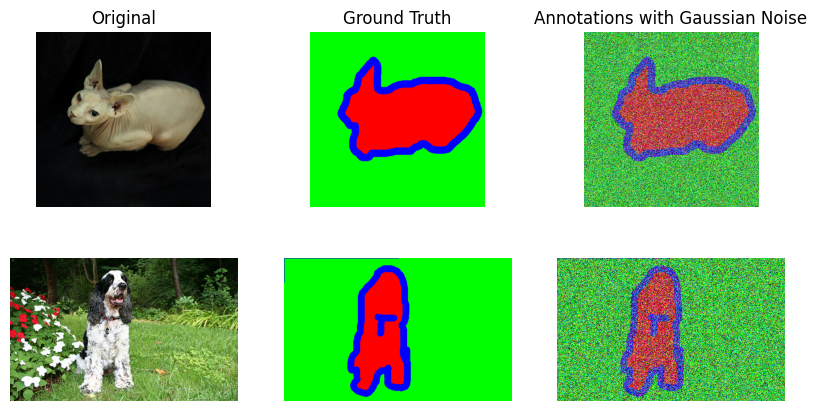
\includegraphics[width=0.7\textwidth]{Cap2/Figures/naive_gaussian_noise.png}
  \caption{Example of a noisy mask generated by naively introducing random
  noise into a ground truth mask. Morphological consistency is lost.}
  \label{fig:noisy_masks}
\end{figure}

For this reason, a more sophisticated approach was needed to create
datasets with emulated noisy annotations. The approach used here was
to use a pre-trained U-Net model to produce a good enough segmentation
of the image, which was then used to produce a ``noisy'' annotation by
introducing random noise into the last encoder layers of the model, thus
preserving the morphological consistency of the original annotation.
This strategy works since slight modifications introduced into
the encoder layers weights, somehow resemble conceptual disturbances with
respect to the original ground truth label, which kind of emulates
the cultural behavior of having a different interpretation of the
image, either for having a different level of expertise or for having a
different point of view or school of thought. The first encoding layers
were not modified, since it is expected human labelers would agree on the
most fundamental structures (analog to extracted features from initial
convolutional layers) in a similar way, thus preserving the morphological
consistency of the original annotation.

In this way, the level of ``disturbance'' with respect to the ground
truth for an emulated annotator can be controlled by the level of
noise introduced into the weights of the last encoder layers, thus:

\begin{equation}
  \mathbf{W}_{noisy} = \mathbf{W}_{original} + \mathcal{N}(0, \sigma^2)
\end{equation}

where $\mathbf{W}_{original}$ represents the original weights of the
last encoder layers, $\mathcal{N}(0, \sigma^2)$ is a Gaussian
distribution with mean 0 and variance $\sigma^2$, and
$\mathbf{W}_{noisy}$ are the resulting noisy weights. The variance
$\sigma^2$ controls the level of noise introduced, and thus the
degree of disturbance in the resulting segmentation masks.

\subsubsection{Oxford-IIIT Pet Dataset}

Using the techniques described above, the Oxford-IIIT Pet Dataset
\cite{ParkhiEtAl2012} was used to create a dataset with emulated noisy
annotations. The almost perfectly uniform distribution of the dataset classes
makes it an ideal playground dataset for testing segmentation models
with a high degree of confidence in the ground truth annotations, at
the same time that cats and dogs are a common sight in the daily life of
most people, making it easier to find a labeler that is able to annotate
the images with a high degree of accuracy, which facilitates model
initial debugging. Figure \ref{fig:oxford_iii_overview} shows an example
of the annotations in the original dataset.

\begin{figure}[h]
  \centering
  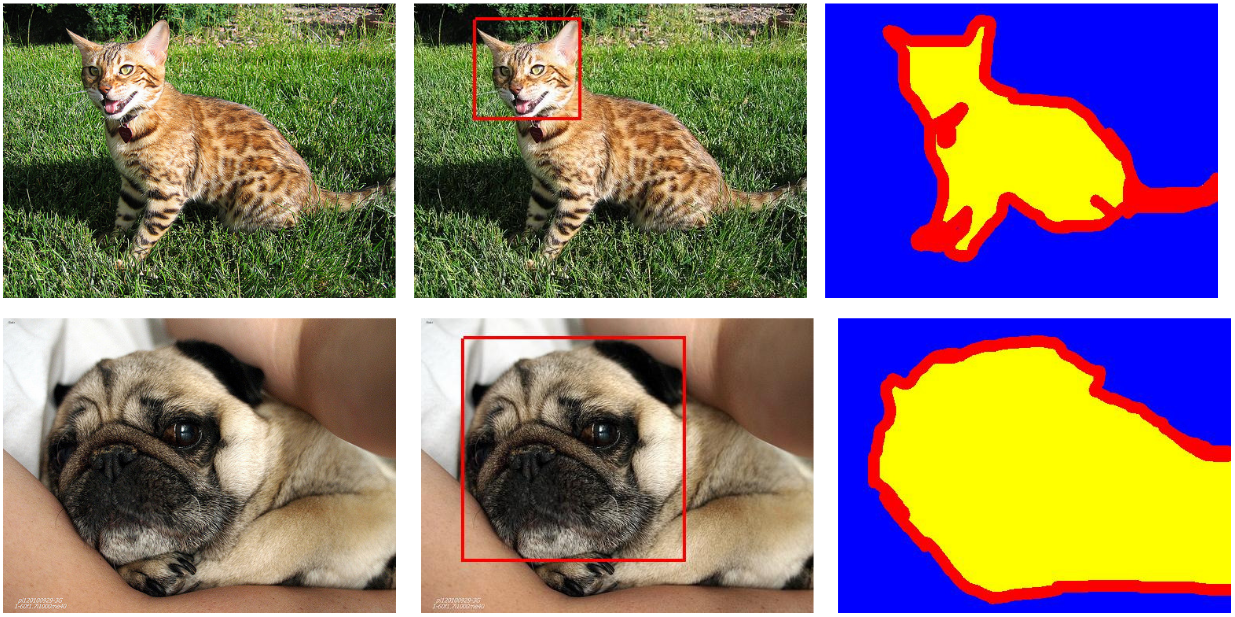
\includegraphics[width=0.7\textwidth]{Cap2/Figures/oxford_iii_overview.png}
  \caption{Annotations in the Oxford-IIIT Pet data. From left
    to right: pet image, head bounding box, and trimap segmentation
    (blue: background region; red: ambiguous region; yellow: foreground
  region).}
  \label{fig:oxford_iii_overview}
\end{figure}

With the application of the encoder layer weight perturbation technique,
the resulting noisy masks are shown in Figure
\ref{fig:enhanced_disturbances}. It can be seen that the
morphological consistency is preserved, even though the resulting
masks are far from the ground truth annotations, which goes perfectly
well for testing the robustness of the models against noisy
annotations in crowdsourcing-like scenarios.
\begin{figure}[h]
  \centering
  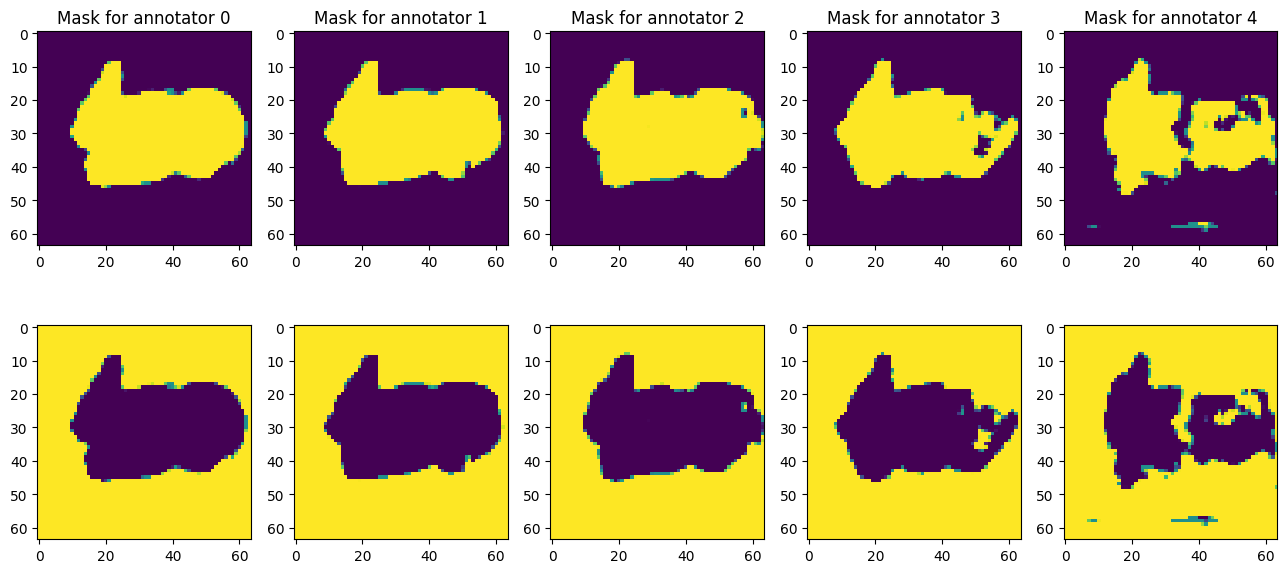
\includegraphics[width=0.8\textwidth]{Cap2/Figures/enhanced_disturbances.png}
  \caption{Noisy mask generated by enhancing the disturbances
    in the encoder layers weights for the Oxford-IIIT Pet Dataset.
    Morphological consistency is preserved. From left to right, SNR
  levels of noise in the encoder layer are 10, 5, 2, 0, -5 dB.}
  \label{fig:enhanced_disturbances}
\end{figure}

\subsection{Real histopathology datasets}

\subsubsection{Multi-Stain Breast Cancer Histological Dataset}

The Multi-Stain Breast Cancer Histological Dataset
\cite{WeitzEtAl2023} represents one of the largest publicly available
collections of whole slide images (WSIs) from surgical resection
specimens of primary breast cancer patients. This dataset is
particularly valuable for our work because it contains matched pairs
of H\&E and IHC-stained tissue sections from the same tumor, with a
total of 4,212 WSIs from 1,153 patients. The IHC stains include
important biomarkers such as ER, PGR, HER2, and KI67, which are
routinely used in breast cancer diagnosis and treatment planning
(more on staining techniques in Section \ref{sec:staining_techniques}).

The dataset's relevance to our work stems from several key aspects.
The matched H\&E and IHC stains allow for studying the consistency of
segmentation across different staining modalities, which is crucial
for understanding how different visualization methods affect
annotation quality. With 1,153 patients, the dataset provides a
robust foundation for training and evaluating segmentation models in
a real-world clinical setting. The inclusion of routine diagnostic
cases makes the dataset representative of actual clinical practice,
where variations in staining quality and tissue preparation are
common. Furthermore, the multiple biomarker stains (ER, PGR, HER2,
KI67) enable the study of how different tissue characteristics affect
segmentation performance and annotator agreement.

This dataset serves as an ideal testbed for our crowdsourced
segmentation approach. It allows us to evaluate how different
staining modalities affect annotator performance and agreement, while
also providing insights into the relationship between tissue
characteristics and segmentation difficulty. The dataset's
comprehensive nature enables validation of our models' performance
across different biomarker expressions and assessment of the
generalizability of our approach to real-world clinical data.

\begin{figure}[h]
  \centering
  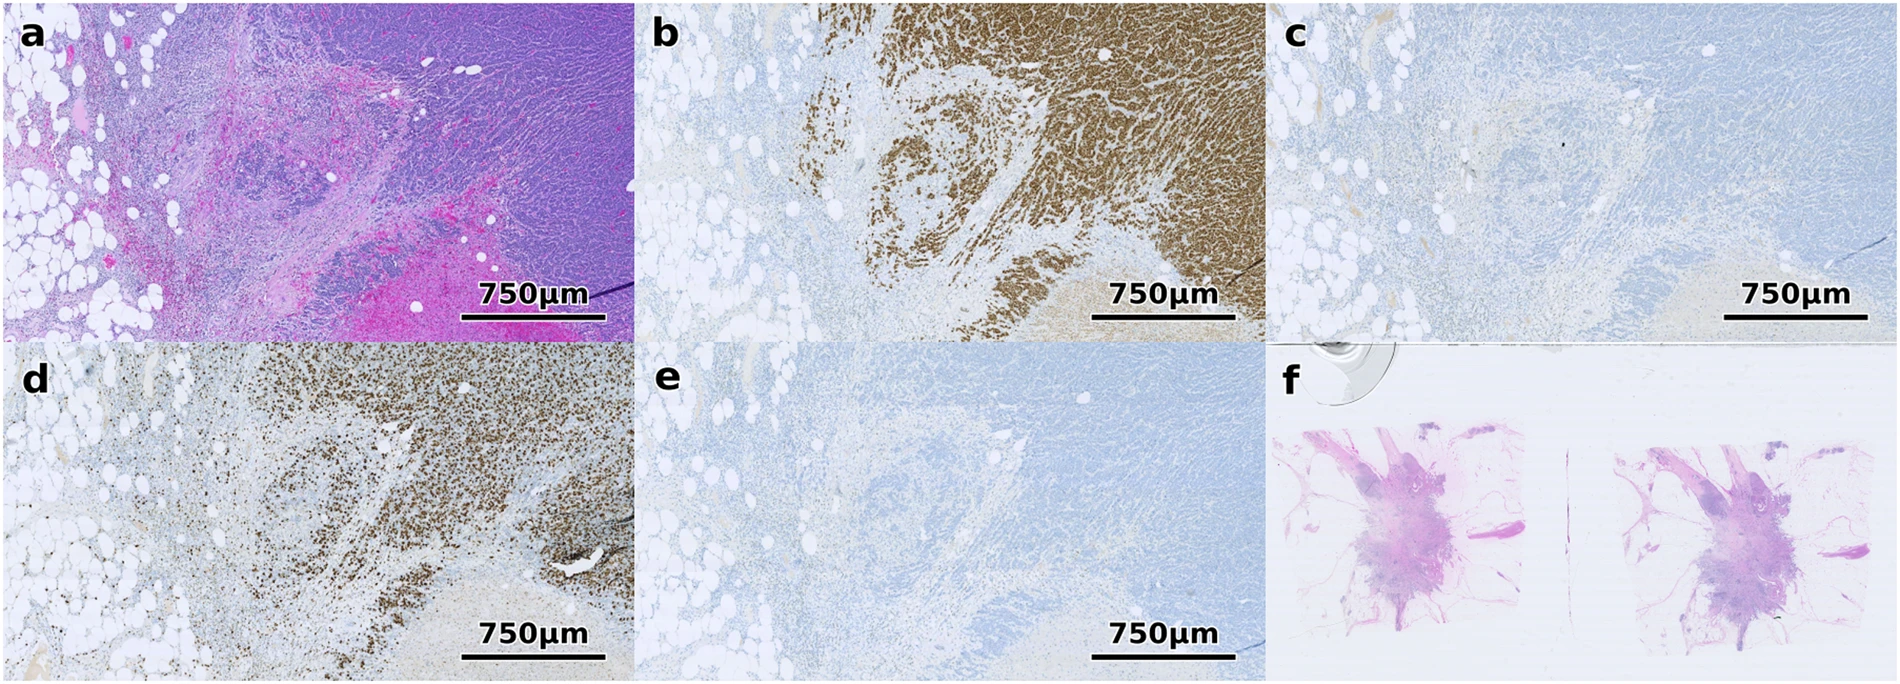
\includegraphics[width=0.7\textwidth]{Cap2/Figures/staining_comparison.png}
  \caption{Different staining techniques obtained from multi-stain
    breast cancer dataset \cite{WeitzEtAl2023}. (a) shows H\&E, (b) ER,
    (c) HER2, (d) Ki67 and (e) PGR. (f) shows an example of a \gls{WSI}
  that was excluded since it contains multiple tissue sections.}
  \label{fig:weitz_dataset_overview}
\end{figure}

\subsubsection{Structured Crowdsourcing Dataset for Histology Images}

The dataset presented by \cite{AmgadEtAl2019} is particularly
relevant to our work as it represents one of the first systematic
studies of crowdsourced annotations in histopathology. The authors
recruited 25 participants with varying levels of expertise (from
senior pathologists to medical students) to delineate tissue regions
in 151 breast cancer slides using the Digital Slide Archive platform,
resulting in over 20,000 annotated tissue regions.

Key aspects of this dataset make it valuable for our work. The
systematic evaluation of inter-participant discordance revealed
varying levels of agreement across different tissue classes, with low
discordance for tumor and stroma, and higher discordance for more
subjectively defined or rare tissue classes. The inclusion of
feedback from senior participants helped in curating high-quality
annotations, demonstrating that fully convolutional networks trained
on these crowdsourced annotations can achieve high accuracy (mean
AUC=0.945). The dataset also provides evidence that the scale of
annotation data significantly improves image classification accuracy.

This dataset is particularly valuable for our work because it
provides crucial insights into how annotator expertise affects
segmentation quality. It demonstrates the feasibility of using
crowdsourced annotations for training accurate segmentation models,
showing that even with varying levels of expertise, aggregated
annotations can produce reliable ground truth. The dataset includes a
systematic analysis of inter-annotator agreement, which is crucial
for understanding the challenges in crowdsourced histopathology
segmentation and informing the development of more robust
segmentation approaches.

\begin{figure}[h]
  \centering
  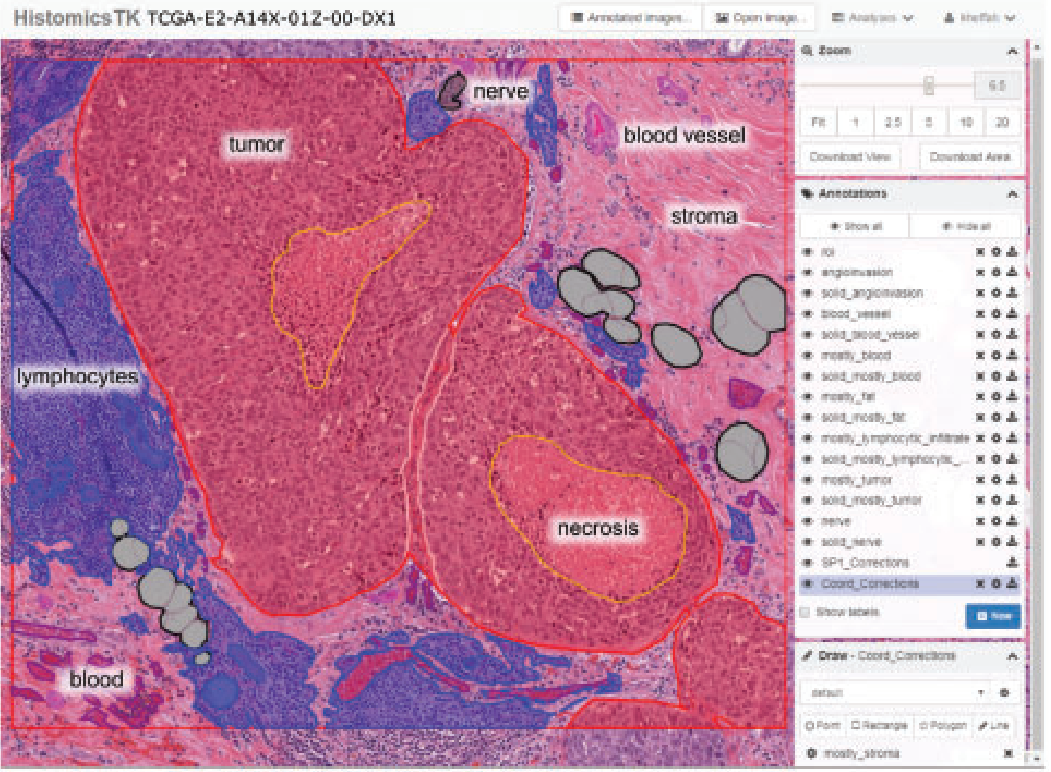
\includegraphics[width=0.8\textwidth]{Cap2/Figures/amgad_histomics_tk.png}
  \caption{Screenshot of the DSA and HistomicsTK web interface while
    creating the crowdsourced annotations for the dataset presented by
  \cite{AmgadEtAl2019}.}
  \label{fig:amgad_histomics_tk}
\end{figure}



% Bibliography
\addcontentsline{toc}{chapter}{Bibliography}
\bibliographystyle{apalike}
%\bibliographystyle{ieeetr}
\bibliography{References,bibliography}

\end{document}